%! Author = yessense
%! Date = 04.02.2022

\documentclass{article}
\usepackage[utf8]{inputenc}
\usepackage{graphicx}
\usepackage{hyperref}
\title{dSprites VSA}
\author{ }
\date{ }

\begin{document}

    \maketitle


    \section{Introduction}

    The goal of this work is to extract the features of the image
    and represent them as multidimensional vectors, which, when
    summed up, will allow you to reconstruct the original image.
    Having started with a single object in the scene, we will try
    to move to a set of several objects.


    \section{Dataset}

    The task consists of three consecutive steps for each of
    which a different dataset was created.

    \subsection{Disentanglement Dataset}
    The work is based on the dataset dsprites \autoref{fig:dsprites_example}
    This dataset contains paired images from the dataset
    dSprites, which differ in one of the following features \autoref{tab:features}.
    An example of pairwise images in a dataset can be seen in the \autoref{fig:disentanglement_dsprites}

    \begin{table}[ht]
        \centering
        \caption{List of features}
        \label{tab:features}
        \begin{tabular}[t]{ll}
            \hline
            Type        & Description                          \\
            \hline
            Shape       & square, ellipse, heart               \\
            Scale       & 6 values linearly spaced in [0.5, 1] \\
            Orientation & 40 values in [0, 2 pi]               \\
            Position X  & 32 values in [0, 1]                  \\
            Position Y  & 32 values in [0, 1]                  \\
            \hline
        \end{tabular}
    \end{table}

    \begin{figure}[t]
        \begin{minipage}[t]{0.32\textwidth}
            \centering
            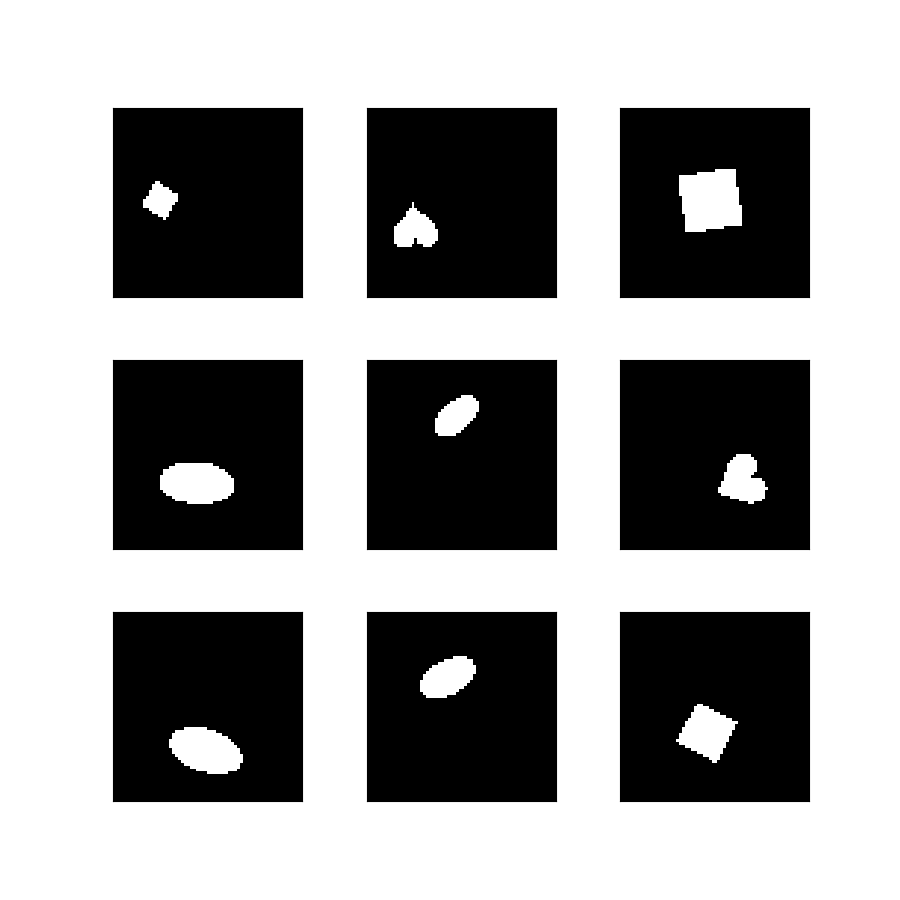
\includegraphics[width=\textwidth]{img/dsprites}
            \caption{Example of images from dSprites dataset}
            \label{fig:dsprites_example}
        \end{minipage}\hfill
        \begin{minipage}[t]{0.32\textwidth}
            \centering
            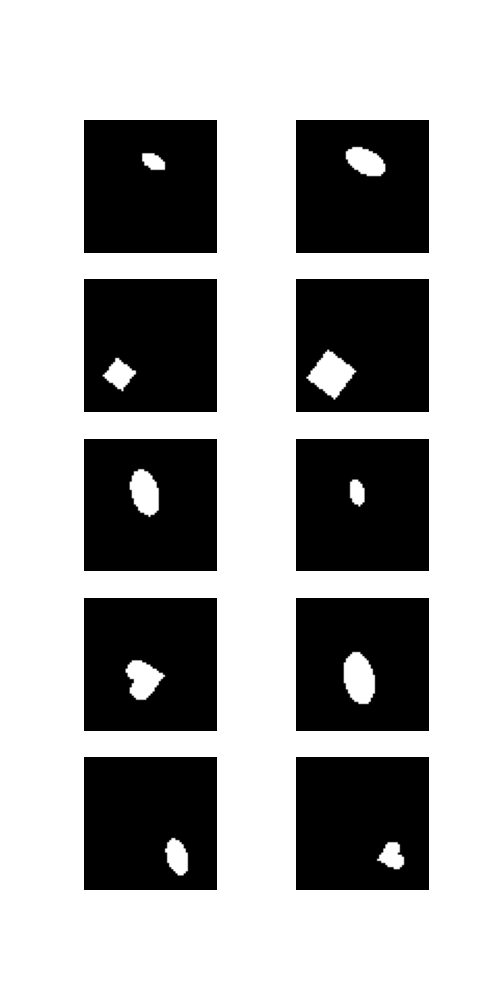
\includegraphics[width=0.5\textwidth]{img/dataset1}
            \caption{Example of paired images in Disentanglement Dataset}
            \label{fig:disentanglement_dsprites}
        \end{minipage}\hfill
        \begin{minipage}[t]{0.32\textwidth}
            \centering
            
\includegraphics[width=0.20\textwidth]{img/multi-dsprites}
            \caption{Example of collected scenes in the multidsprites dataset}
            \label{fig:multi_dsprites}
        \end{minipage}
    \end{figure}

    \subsection{Multi-dsprites dataset}
    Dataset consists of 2 to 5 non-overlapping figures from dSprites dataset.
    An example of such images on \autoref{fig:multi_dsprites}
\end{document}
